\chapter{Implementation}

\section{System Architecture}

The AIT Policy Validation System follows a three-layer architecture:

\begin{figure}[h]
\centering
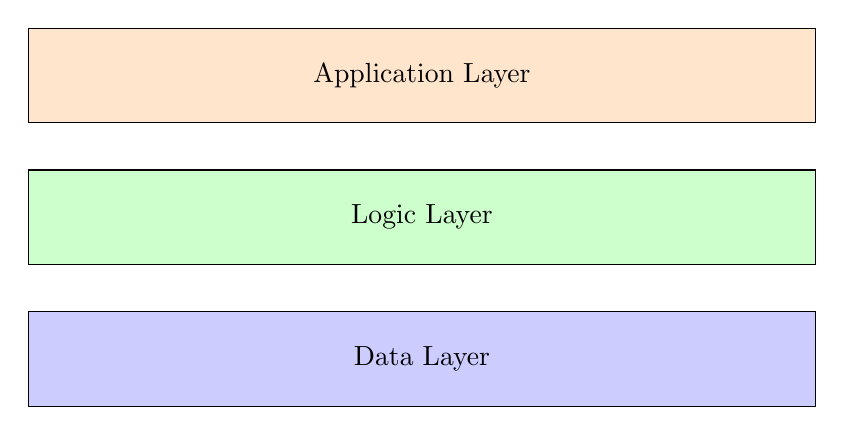
\begin{tikzpicture}[
    node distance=1cm,
    layer/.style={rectangle, draw, minimum width=10cm, minimum height=1.2cm, fill=#1},
    component/.style={rectangle, draw, minimum width=2.8cm, minimum height=0.8cm, fill=white}
]
    % Layers
    \node[layer=blue!20] (data) at (0,0) {Data Layer};
    \node[layer=green!20] (logic) at (0,1.8) {Logic Layer};
    \node[layer=orange!20] (app) at (0,3.6) {Application Layer};
    
    % Components - simplified representation
\end{tikzpicture}
\caption{System Architecture}
\end{figure}

\subsection{Components}

\begin{description}
    \item[PostgreSQL Database] Stores student and financial data
    \item[Ontop Virtual Knowledge Graph] Maps relational data to RDF via OBDA
    \item[GraphDB] RDF triple store and SPARQL endpoint
    \item[SHACL Validator] Executes validation rules (PySHACL)
    \item[Explanation Generator] (Future) LLM-based explanation of violations
\end{description}

\section{Complete Worked Example}

This section demonstrates the complete transformation pipeline from a real AIT policy to a validated SHACL shape.

\subsection{Step 1: Original Policy Statement}

\begin{quote}
\textit{``For self-support students and holders of externally-managed scholarships: first semester/term fees must be paid in advance and/or fully paid upon enrolment, otherwise they will not be allowed to register.''}

\hfill -- AIT Credit Policy FB-6-1-1, Section II.1(1)
\end{quote}

\subsection{Step 2: Policy Analysis}

\begin{table}[h]
\centering
\caption{Annotation of Example Policy}
\begin{tabular}{ll}
\toprule
Dimension & Value \\
\midrule
Syntactic Structure & Complex (condition + consequence) \\
Deontic Type & Obligation (must) \\
Quantification & Universal (all self-support students) \\
Conditional Structure & Single condition \\
Temporal Elements & Deadline (upon enrolment) \\
Entities & Student, Fee, Registration \\
Ambiguity & ``in advance'' is vague \\
\bottomrule
\end{tabular}
\end{table}

\subsection{Step 3: Disambiguation}

\textbf{Original Ambiguity}: ``paid in advance and/or fully paid upon enrolment''

\textbf{Interpretation}: The fee must be fully paid by the time of registration. ``In advance'' and ``upon enrolment'' are treated as equivalent for this rule.

\textbf{Simplified Statement}: Self-support students must have paid their first semester tuition fees to be eligible for registration.

\subsection{Step 4: First-Order Logic Representation}

\begin{equation}
\forall x, o \left[
\begin{array}{l}
\text{Student}(x) \land \text{Type}(x, \text{``Self-Support''}) \land \\
\text{Status}(x, \text{``Enrolled''}) \land \text{Obligation}(o) \land \\
\text{hasObligation}(x, o) \land \text{Type}(o, \text{``TuitionFee''}) \land \\
\neg\text{Paid}(o)
\end{array}
\rightarrow \text{Violation}(x) \right]
\end{equation}

\textbf{Reading}: For any student $x$ with obligation $o$, if $x$ is a self-support student who is enrolled, and $o$ is an unpaid tuition fee obligation of $x$, then $x$ is in violation.

\subsection{Step 5: Ontology Terms}

\begin{table}[h]
\centering
\caption{Ontology Mapping}
\begin{tabular}{lll}
\toprule
FOL Term & Ontology URI & Type \\
\midrule
Student(x) & ait:Student & Class \\
Type(x, ``Self-Support'') & ait:hasStudentType & DataProperty \\
Status(x, ``Enrolled'') & ait:hasEnrollmentStatus & DataProperty \\
Obligation(o) & ait:Obligation & Class \\
hasObligation(x, o) & ait:hasFinancialObligation & ObjectProperty \\
Type(o, ``TuitionFee'') & ait:hasObligationType & DataProperty \\
Paid(o) & ait:isPaid & DataProperty \\
\bottomrule
\end{tabular}
\end{table}

\subsection{Step 6: SHACL Shape}

\begin{lstlisting}[style=turtle, caption={Tuition Compliance SHACL Shape}]
@prefix ait: <http://ait.ac.th/ontology#> .
@prefix sh:  <http://www.w3.org/ns/shacl#> .
@prefix xsd: <http://www.w3.org/2001/XMLSchema#> .

ait:TuitionComplianceShape
  a sh:NodeShape ;
  sh:targetClass ait:Student ;
  sh:sparql [
    a sh:SPARQLConstraint ;
    sh:message "Self-Support students must pay 
                tuition fees to be enrolled." ;
    sh:select """
      PREFIX ait: <http://ait.ac.th/ontology#>
      PREFIX xsd: <http://www.w3.org/2001/XMLSchema#>
      
      SELECT $this
      WHERE {
        $this a ait:Student .
        $this ait:hasStudentType "Self-Support" .
        $this ait:hasEnrollmentStatus "Enrolled" .
        $this ait:hasFinancialObligation ?obl .
        ?obl ait:hasObligationType "TuitionFee" .
        ?obl ait:isPaid "false"^^xsd:boolean .
      }
    """ ;
  ] .
\end{lstlisting}

\subsection{Step 7: Test Data}

\textbf{Compliant Case (Should Pass)}:
\begin{lstlisting}[style=turtle]
ait:student_001 a ait:Student ;
    ait:hasStudentType "Self-Support" ;
    ait:hasEnrollmentStatus "Enrolled" ;
    ait:hasFinancialObligation ait:obl_001 .

ait:obl_001 a ait:Obligation ;
    ait:hasObligationType "TuitionFee" ;
    ait:isPaid true .
\end{lstlisting}

\textbf{Violation Case (Should Fail)}:
\begin{lstlisting}[style=turtle]
ait:student_002 a ait:Student ;
    ait:hasStudentType "Self-Support" ;
    ait:hasEnrollmentStatus "Enrolled" ;
    ait:hasFinancialObligation ait:obl_002 .

ait:obl_002 a ait:Obligation ;
    ait:hasObligationType "TuitionFee" ;
    ait:isPaid false .
\end{lstlisting}

\subsection{Step 8: Validation Result}

When running SHACL validation:

\begin{itemize}
    \item \textbf{student\_001}: Conforms (no violations)
    \item \textbf{student\_002}: Violation detected
    \begin{itemize}
        \item Focus Node: ait:student\_002
        \item Message: ``Self-Support students must pay tuition fees to be enrolled.''
    \end{itemize}
\end{itemize}

\section{Tool Chain}

\begin{table}[h]
\centering
\caption{Tools Used in Implementation}
\begin{tabular}{lll}
\toprule
Tool & Purpose & Version \\
\midrule
Prot\'eg\'e & Ontology editing & 5.5+ \\
GraphDB & RDF triple store & 11.1.1 \\
Ontop & Virtual Knowledge Graph & 5.1+ \\
PySHACL & SHACL validation (Python) & 0.25+ \\
PostgreSQL & Relational database & 15+ \\
SHACL2FOL & FOL verification & Latest \\
\bottomrule
\end{tabular}
\end{table}

\section{Additional Implemented Rules}

\subsection{Accommodation Overdue Rule}

\textbf{Policy}: ``If accommodation and other fees remain unpaid beyond two months, a student's status shall be `suspended/dismissed due to financial inability'.''

\textbf{SHACL Implementation}: See Appendix C for full shape definition.

\textbf{Test Cases}: Three test cases created (compliant, 30-day overdue, 90-day overdue).
